\documentclass[tikz]{standalone}
\usepackage[utf8]{inputenc} 			
\usepackage[norsk]{babel}
\usetikzlibrary{shapes.geometric, arrows}

\tikzstyle{startstop} = [rectangle, rounded corners, minimum width=3cm, minimum
height=1cm,text centered, draw=black, fill=red!30] \tikzstyle{io} = [trapezium,
trapezium left angle=70, trapezium right angle=110, minimum width=3cm, minimum
height=1cm, text centered, draw=black, fill=blue!30] \tikzstyle{process} =
[rectangle, minimum width=3cm, minimum height=1cm, text centered, draw=black,
fill=orange!30] \tikzstyle{decision} = [diamond, minimum width=3cm, minimum
height=1cm, text centered, draw=black, fill=green!30]

\tikzstyle{arrow} = [thick,->,>=stealth]

\begin{document}

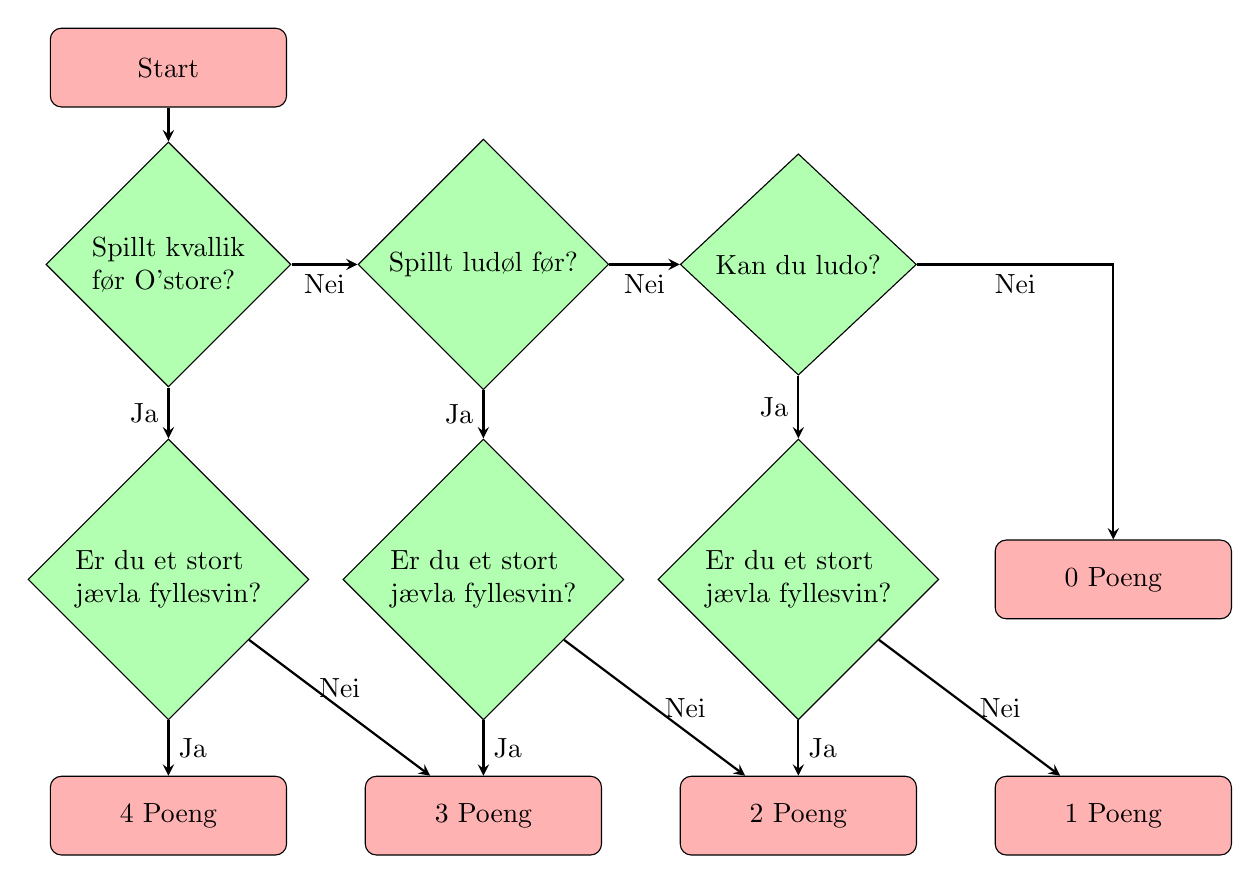
\begin{tikzpicture}[node distance=2cm]

  \node (start) [startstop] {Start};
  \node (dec1) [decision, below of=start, yshift=-0.5cm, align=left] {Spillt kvallik \\ før O'store?};
  \node (dec2) [decision, below of=dec1, yshift=-2cm, align=left] {Er du et stort \\ jævla fyllesvin?};

  \node (dec3) [decision, right of=dec1, xshift=2cm] {Spillt ludøl før?};
  \node (dec4) [decision, below of=dec3, yshift=-2cm, align=left] {Er du et stort \\ jævla fyllesvin?};
  
  \node (dec5) [decision, right of=dec3, xshift=2cm] {Kan du ludo?};
  \node (dec6) [decision, below of=dec5, yshift=-2cm, align=left] {Er du et stort \\ jævla fyllesvin?};

  % \node (dec4) [decision, right of=dec1, xshift=2cm] {Spillt ludøl før?};
  \node (stop1) [startstop, below of=dec2, yshift=-1cm] {4 Poeng};
  \node (stop2) [startstop, below of=dec4, yshift=-1cm] {3 Poeng};
  \node (stop3) [startstop, below of=dec6, yshift=-1cm] {2 Poeng};
  \node (stop4) [startstop, right of=stop3, xshift = 2cm] {1 Poeng};
  \node (stop5) [startstop, right of=dec6, xshift = 2cm] { 0 Poeng};

  \draw [arrow] (start) -- (dec1);
  \draw [arrow] (dec1) -- node[anchor=east] {Ja} (dec2);
  \draw [arrow] (dec1) -- node[anchor=north] {Nei} (dec3);
  \draw [arrow] (dec3) -- node[anchor=north] {Nei} (dec5);
  \draw [arrow] (dec4) -- node[anchor=west] {Nei} (stop3);
  \draw [arrow] (dec3) -- node[anchor=east] {Ja} (dec4);
  \draw [arrow] (dec5) -- node[anchor=east] {Ja} (dec6);
  \draw [arrow] (dec6) -- node[anchor=west] {Ja} (stop3);
  \draw [arrow] (dec6) -- node[anchor=west] {Nei} (stop4);

  \node (temp) [right of=dec5, xshift=2cm] {};

  \draw[arrow] (dec5) -- node[anchor=north] {Nei} (temp.center) -- (stop5);
  
  \draw [arrow] (dec2) -- node[anchor=west] {Ja} (stop1);
  
  \draw [arrow] (dec2) -- node[anchor=south] {Nei} (stop2);
  \draw [arrow] (dec4) -- node[anchor=west] {Ja} (stop2);

\end{tikzpicture}

\end{document}
